\section{Three easy applications of Bayes's theorem:}

\begin{enumerate}[label=\textbf{\Alph*}.]
    \item Suppose supernovae follow a poisson distribution with an unknown rate $R$. Calculate and plot the posterior distribution for $R$, given an observation of 4 supernovae in 10 centuries, using (a) a prior uniform in $R$ and (b) a prior uniform in $\log_{10}(R)$.

    Remember Bayes's theorem:
    \begin{align*}
        \text{posterior} = \frac{\text{likelihood} \times \text{prior}}{\text{probability of data}}
    \end{align*}

    The priors: 
    \begin{itemize}
        \item Uniform in $R$, but we're not given bounds... Suppose it goes from some $n$ to $m$. $$P(R) = \frac{1}{m-n}.$$
        \item Uniform in $\log_{10}(R)$: use $P(x)dx = P(f(x))df(x)$ to get 
        \begin{align*}
            P(R) &= P(\log_{10}(R)) \frac{d\log_{10}(R)}{dR} \\
            &= \frac{\ln(10)}{\ln(m)-\ln(n)} \frac{1}{\ln(10)R} \\
            &= \frac{1}{\ln(m)-\ln(n)} \frac{1}{R} \\
        \end{align*}
    \end{itemize}

    Likelihood: Poisson distribution ($T$ = 1000 years)
    \begin{align*}
        P(k|R) = \frac{e^{-RT}(RT)^k}{k!}
    \end{align*}

    Probability of Data:
    \begin{align*}
        P(k) &= \int P(R) P(k|R) dR \\
    \end{align*}
    for uniform $R$,
    \begin{align*}
        P(k) &= \int_0^\infty \frac{1}{m-n} \frac{e^{-RT}(RT)^k}{k!} dR \\
        &= \frac{1}{m-n}\frac{1}{k!} \int_0^\infty e^{-RT}(RT)^k dR \\
        &= \frac{1}{m-n}\frac{1}{k!}\frac{1}{T} \int_0^\infty e^{-\lambda}(\lambda)^k d\lambda \\
        &= \frac{1}{m-n}\frac{1}{k!}\frac{1}{T} k! \\
        &= \frac{1}{m-n}\frac{1}{T} \\
    \end{align*}
    or for uniform $\log_{10}(R)$
    \begin{align*}
        P(k) &= \int_0^\infty \frac{1}{\ln(m)-\ln(n)}\frac{1}{R} \frac{e^{-RT}(RT)^k}{k!} dR \\
        &= \frac{1}{\ln(m)-\ln(n)} \int_0^\infty T \frac{1}{RT} \frac{e^{-RT}(RT)^k}{k!} dR \\
        &= \frac{1}{\ln(m)-\ln(n)} \int_0^\infty \frac{e^{-\lambda}(\lambda)^{k-1}}{k!} d\lambda &[\lambda = RT]\\
        &= \frac{1}{\ln(m)-\ln(n)}\frac{1}{k} \\
    \end{align*}
    
    Now calculate posteriors:

    Uniform $R$:
    \begin{align*}
        P(R|k) &= \frac{P(k|R)P(R)}{P(k)}\\
        &= \frac{\frac{e^{-RT}(RT)^k}{k!}\frac{1}{m-n}}{\frac{1}{m-n}\frac{1}{T}}\\
        &= \frac{\frac{e^{-RT}(RT)^k}{k!}}{\frac{1}{T}}\\
        &= \frac{Te^{-RT}(RT)^k}{k!}\\
    \end{align*}

    Uniform $\log_{10}(R)$
    \begin{align*}
        P(R|k) &= \frac{P(k|R)P(R)}{P(k)}\\
        &= \frac{\frac{e^{-RT}(RT)^k}{k!}\frac{1}{\ln(m)-\ln(n)} \frac{1}{R}}{\frac{1}{\ln(m)-\ln(n)}\frac{1}{k}}\\
        &= \frac{Te^{-RT}(RT)^{k-1}}{(k-1)!}\\
    \end{align*}

    Plot of these distributions:

    \begin{figure}[H]
        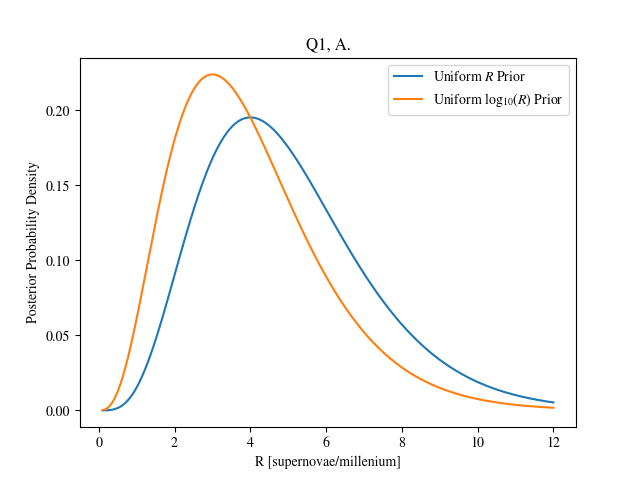
\includegraphics[width=\textwidth]{q1_a.png}
    \end{figure}

    \item Measurements are drawn from a uniform distribution spanning the interval (0, m). The probability of getting a measurement outside of this range is zero. The endpoint m is not well-known, but a prior experiment yields a Gaussian prior of m = 3 +/- 1. You take three measurements, getting values of 2.5, 3.1, and 2.9. Use Bayes' theorem to calculate and plot the new probability distribution for m.

    Likelihood: if our model is a uniform distribution on $[0,m]$ and we have independent measurements (which I think we can assume for this question, right?), then $P(D|m) = \frac{1}{m^3}$ if $m \geq 3.1$, $=0$ otherwise. That's the product of three uniform probabilities.

    Prior (Gaussian, $\mu=3, \sigma=1$): $P(m) = \frac{1}{\sqrt{2\pi}}e^{-\frac{(m-3)^2}{2}}$.

    Probability of Data:
    \begin{align}
        P(D) &= \int_0^\infty P(m) P(D|m) dm \\
        &= \int_{3.1}^\infty \frac{1}{\sqrt{2\pi}}e^{-\frac{(m-3)^2}{2}} \frac{1}{m^3} dm \\
    \end{align}

    Posterior:
    \begin{align*}
        P(m|D) &= \frac{P(D|m)P(m)}{P(D)}\\
        &= \frac{\frac{1}{m^3}\frac{1}{\sqrt{2\pi}}e^{-\frac{(m-3)^2}{2}}}{\int_{3.1}^\infty \frac{1}{\sqrt{2\pi}}e^{-\frac{(m'-3)^2}{2}} \frac{1}{m'^3} dm'} &[m \ge 3.1, \text{ else }0]\\
        &= \frac{\frac{1}{m^3}e^{-\frac{(m-3)^2}{2}}}{\int_{3.1}^\infty e^{-\frac{(m'-3)^2}{2}} \frac{1}{m'^3} dm'} &[m \ge 3.1, \text{ else }0]\\
    \end{align*}

    Plot:
    \begin{figure}[H]
        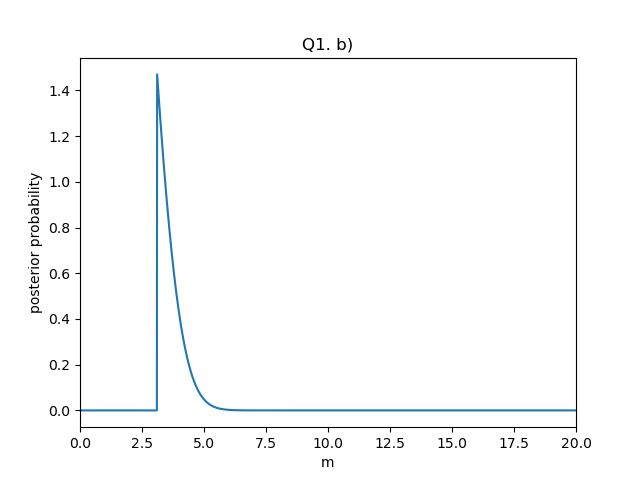
\includegraphics[width=\textwidth]{q1_b.png}
    \end{figure}

    \item Consider a person considering whether or not to launch a rocket with a possible malfunctioning component. In the control centre there is a warning light that is not completely reliable. During launch the warning light doesn't go on. From a costs standpoint, should she abort the mission or not? Compute and compare the expected cost of launching to the expected cost of aborting, given that the light didn't go on.
    \begin{itemize}
        \item $P(\text{light on}|\text{malfunction}) = 1/2$, $P(\text{light on}|\text{no malfunction}) = 1/3$
        \item $C(\text{no launch, no malfunction}) = 2M$, $C(\text{launch, malfunction}) = 5M$
        \item $C(\text{no launch, malfunction}) = C(\text{launch, no malfunction}) = 0$
        \item $\operatorname{Prior}(\text{malfunction}) = 2/5$
    \end{itemize}

    Let $F$ denote component failure, $L$ denote the light being on, and $A$ denote a launch (since $L$ was taken).

    Priors: $P(F) = \frac{2}{5}, P(\neg F) = \frac{3}{5}$.

    Likelihood of observing data (no light): $P(\neg L|F) = \frac{1}{2}, P(\neg L|\neg F) = \frac{2}{3}$.

    Probability of seeing our data (no light):
    \begin{align*}
        P(\neg L) &= P(\neg L|F)P(F) + P(\neg L|\neg F)P(\neg F) = \frac{3}{5} \\
    \end{align*}

    Posteriors:
    \begin{align*}
        P(F|\neg L) &= \frac{P(F) P(\neg L | F)}{P(\neg L)}
        = \frac{\frac{2}{5} \frac{1}{2}}{\frac{3}{5}} 
        = \frac{1}{3} \\
        P(\neg F|\neg L) &= 1 - P(F|\neg L)
        = \frac{2}{3} \\
    \end{align*}

    Costs:
    \begin{align*}
        C(A) &= P(F|\neg L)C(F|A) + P(\neg F|\neg L)C(\neg F|A)\\
        &= \frac{1}{3}(5M) + \frac{2}{3}(0)\\
        &= \frac{5}{3}M\\
    \end{align*}
    \begin{align*}
        C(\neg A) &= P(F|\neg L)C(F|\neg A) + P(\neg F|\neg L)C(\neg F|\neg A)\\
        &= \frac{1}{3}(0) + \frac{2}{3}(2M)\\
        &= \frac{4}{3}M\\
    \end{align*}

    The expected cost of not launching is less, so from a cost standpoint, the mission should be aborted, and the rocket makers should probably invest in a better warning light for next time.

\end{enumerate}
